\documentclass[t]{beamer}
\usetheme{Copenhagen}
\setbeamertemplate{headline}{} % remove toc from headers
\beamertemplatenavigationsymbolsempty

\usepackage{amsmath, array, tikz, tcolorbox, bm, tkz-euclide,pgfplots}
\pgfplotsset{compat = 1.16}
\usetkzobj{all}
\everymath{\displaystyle,}

\title{Parabolas}
\author{}
\date{}

\AtBeginSection[]
{
  \begin{frame}
    \frametitle{Objectives}
    \tableofcontents[currentsection]
  \end{frame}
}

\begin{document}

\begin{frame} 
\maketitle
\end{frame}

\section{Identify vertex, focus, and directrix from an equation.} 

\begin{frame}{Parabolas}
If we look at the graph of the quadratic function $f(x) = ax^2 + bx + c$, we obtain what is known as a \emph{parabola}.	\newline\\	\pause

\begin{tcolorbox}[colback=red!10!white, colframe=red!60!black,, title=\textbf{Parabolas}]
The set of all points in the plane that are the same distance from the focus and the directrix line.
\end{tcolorbox}
\end{frame}

\begin{frame}{Parabolas}
\begin{center}
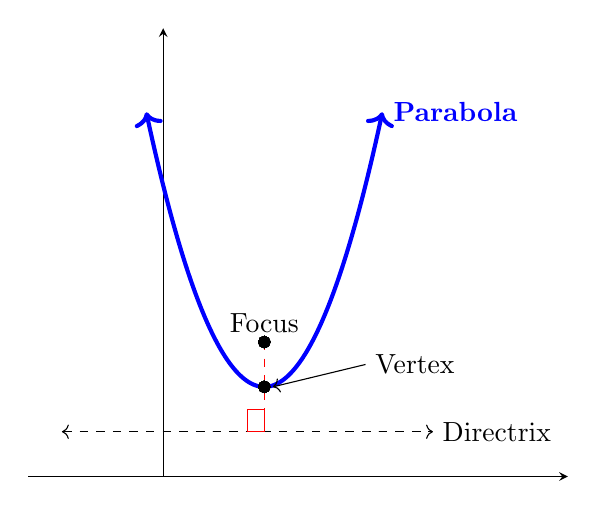
\begin{tikzpicture}
    \begin{axis}[
    axis lines = middle,
    xmin = -4,
    xmax = 12,
    ymin = 0,
    ymax = 10,
    xtick = \empty,
    ytick = \empty]
    \addplot [color=blue, <->, samples=200, domain=-0.5:6.5, line width = 1.5] {2 + 0.5*(x-3)^2} node[right]{\color{blue}{\textbf{Parabola}}};
    \addplot [mark = *] (3, 3) node[above]{Focus};
    \addplot [dashed, <->, samples=200, domain = -3:8] {1} node[right]{Directrix};
    \addplot [mark = *] (3, 2);
    \draw [<-] (3.25,2) -- (6,2.5) node[right]{Vertex};
    \draw [color=red] (3,1) rectangle (2.5,1.5);
    \draw [color=red, dashed] (3,3) -- (3,2) -- (3,1);
    \end{axis}
\end{tikzpicture}
\end{center}
\end{frame}

\begin{frame}{General Form of a Parabola}
The general form of a parabola is the familiar quadratic equation $f(x) = ax^2 + bx + c$.	\newline\\	\pause
The {\color{blue}\textbf{vertex forms}} of a parabola is given below.

\begin{center}
    \setlength{\extrarowheight}{5pt}
    \begin{tabular}{c|c|c}
    &   \textbf{Opens Up or Down}   &   \textbf{Opens Left or Right}    \\  \hline
    &   $y = a(x-h)^2 + k$  &   $x = a(y-k)^2 + h$  \\[5pt]  \hline
    Vertex  &   $(h,k)$ &   $(h,k)$ \\[5pt]  \hline
    Focus   &   $(h,k+p)$ where $a = \frac{1}{4p}$   &   $(h+p,k)$ where $a = \frac{1}{4p}$  \\[5pt] \hline
    Directrix   &   $y = k-p$   &   $x = h-p$   \\
    \end{tabular}
\end{center}
\end{frame}

\begin{frame}{General Form of a Parabola}
\emph{Note}: $p$ is the distance from the focus to the vertex, or the distance from the vertex to the directrix; either interpretation is correct.
\end{frame}

\begin{frame}{Example 1}
Identify the vertex, focus, and directrix for each of the following.    \newline\\  
(a) \quad $ y = 2(x+1)^2 $
\end{frame}


\section{Find the equation given vertex, focus, and/or directrix.}
\section{Convert parabolas between general and vertex form.}

\end{document}